\section{Parameter-efficient fine-tuning}

As we observed in question 1, fine-tuning the entire model can become extremely costly for very large models. In this question, we'll explore more methods for \textit{parameter-efficient fine-tuning}, i.e., methods that enable fine-tuning while creating fewer new parameters and are less prone to overfitting.

\begin{enumerate}[label={3.\alph*}]
    \item \points{3a} {\bf Implement Parameter-efficient Fine Tine}

Finish the implementation for each version of parameter-efficient fine-tuning for GPT-2-Medium in 

\texttt{ft.py:parameters\_to\_fine\_tune()}:

\begin{enumerate}[label=(\roman*)]
    \item \texttt{last}: Fine-tune only the last 2 transformer blocks
    \item \texttt{first}: Fine-tune only first 2 transformer blocks
    \item \texttt{middle}: Fine-tune only middle 2 transformer blocks
\end{enumerate}
This step simply requires selecting the correct subset of parameters for each version listed above in 

\texttt{parameters\_to\_fine\_tune()}. Keep in mind you should be returning an iterable of \texttt{nn.Parameter} here, not \texttt{nn.Module}.
    \item \points{3b} {\bf LoRA}

In addition to selecting only a subset of layers to fine-tune, more sophisticated methods for parameter-efficient fine-tuning exist; one such method is \href{https://arxiv.org/pdf/2106.09685.pdf}{LoRA: Low-rank adaptation}. For each layer $\ell$ in the network, rather than fine-tune the pre-trained weight matrix $W_\ell^0 \in \mathbb{R}^{d_1\times d_2}$ into an arbitrary new weight matrix $W_\ell^{ft}$, LoRA constrains the space of fine-tuned parameters such that $W_\ell^{ft} = W_\ell^0 + AB^\top$, where $A \in \mathbb{R}^{d_1\times p}$ and $B \in \mathbb{R}^{d_2\times p}$, and $p << d_1,d_2$. That is, we force the \textit{difference} between $W_\ell^0$ and $W_\ell^{ft}$ to be rank $p$, keeping $W_\ell^0$ frozen and only fine-tuning the rank-$p$ residual matrix $AB^\top$. We will apply this form of fine-tuning to both the MLP weight matrices and the self-attention weight matrices in the model.

For a single layer, what are the parameter savings we achieve by using LoRA? i.e., what is the ratio of parameters fine-tuned by LoRA (for arbitrary $p$) to the number of parameters in $W_\ell^0$? In terms of $p,d_1,d_2$, when will LoRA provide the greatest savings in newly-created parameters?

    \item \points{3c} {\bf Implement LoRA}

With the information provided in the previous point let us know implement \href{https://arxiv.org/pdf/2106.09685.pdf}{LoRA: Low-rank adaptation}
\begin{enumerate}[label=(\roman*)]
    \item Finish the \texttt{LoRAConv1DWrapper} in \texttt{ft.py}, which wraps a pre-trained Conv1D layer with LoRA parameters. Conv1D is equivalent to a Linear layer; it's a 1D conv because we apply the same linear transform at each time step of the sequence. You can extract the shape of the pre-trained weight matrix from the \texttt{base\_module.weight.shape} tuple. You don't need to worry about biases here, just the low-rank weight matrix residual.
    
    \item Add the corresponding logic for LoRA in \texttt{ft.py:parameters\_to\_fine\_tune()}. Hint: consider using the \texttt{.modules()} function of \texttt{nn.Module} and checking for modules that are an instance of \texttt{LoRAConv1DWrapper}.
    \item Implement the 3-dim version of the loss and accuracy in \texttt{ft.py:get\_loss()} and \texttt{ft.py:get\_acc()}.
    \item Implement batch construction for fine-tuning GPT-2 in function \texttt{ft.py:\allowbreak tokenize\_\allowbreak gpt2\_batch()}. Read the instructions in the code carefully!
    \item Finally, put it all together by filling out the logic for one step of training in \texttt{ft.py:ft\_gpt2()}. Note that we use \textit{gradient accumulation}, meaning that accumulate gradients over \texttt{grad\_accum} steps, and only update our model's parameters after each \texttt{grad\_accum} steps.
\end{enumerate}

\clearpage
    \item {\bf Evaluate}

\begin{enumerate}[label=(\roman*)]
    \item \points{3di} {\bf Run Fine-Tuning with LoRA}

Run fine-tuning for each parameter-efficient fine-tuning method, using $p=4,16$ for LoRA (so, 5 variants in total); run the commands:

{\small \texttt{python3 main.py --task run\_ft --model med --mode first,last,middle,lora4,lora16 \textbackslash \\
\phantom{asdf}--dataset xsum,babi --k 0,1,8,128}}

Plot \textbf{k-shot performance} as \textbf{k is varied} for GPT-2-medium, one plot for each dataset; run the commands:

{\small \texttt{python3 main.py --task plot\_ft --model med --mode first,last,middle,lora4,lora16 \textbackslash \\
\phantom{asdf}--dataset xsum --k 0,1,8,128}}

Plot for the above is as follows:
\begin{center}
    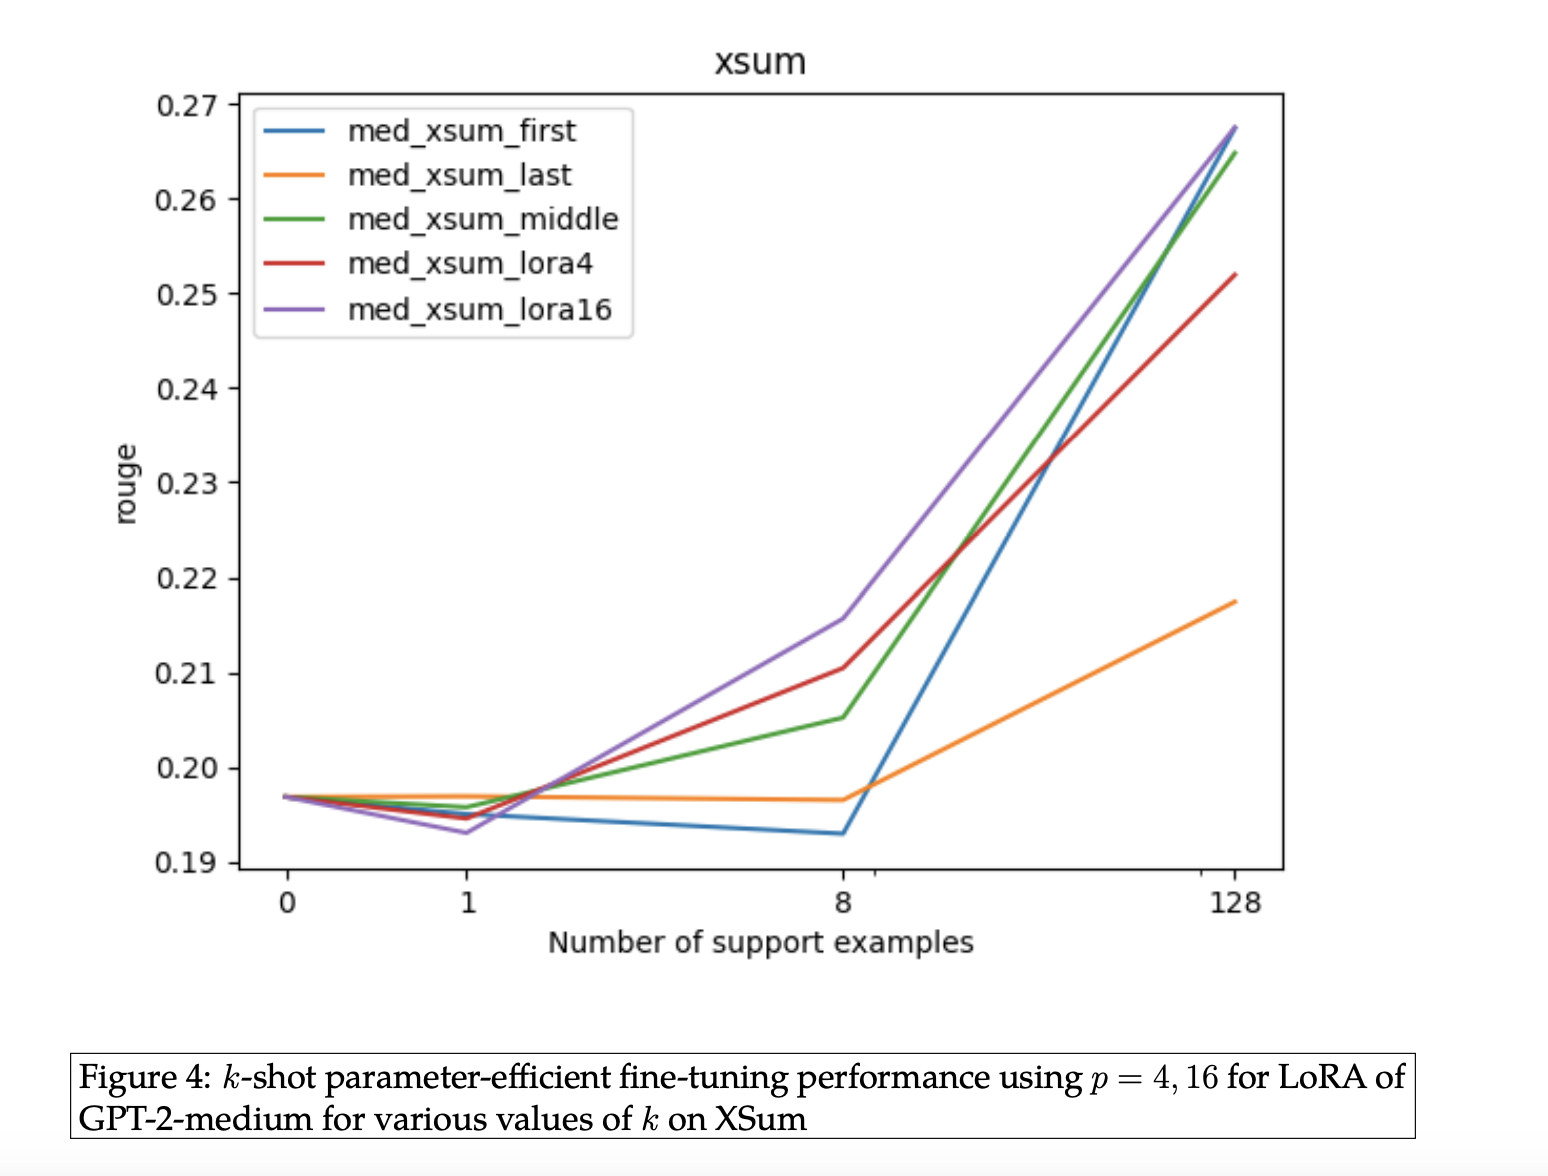
\includegraphics[width=0.75\linewidth]{./figures/parameter-3ci}
\end{center}

{\small \texttt{python3 main.py --task plot\_ft --model med --mode first,last,middle,lora4,lora16 \textbackslash \\
\phantom{asdf}--dataset babi --k 0,1,8,128}}

Plot for the above is as follows:
\begin{center}
    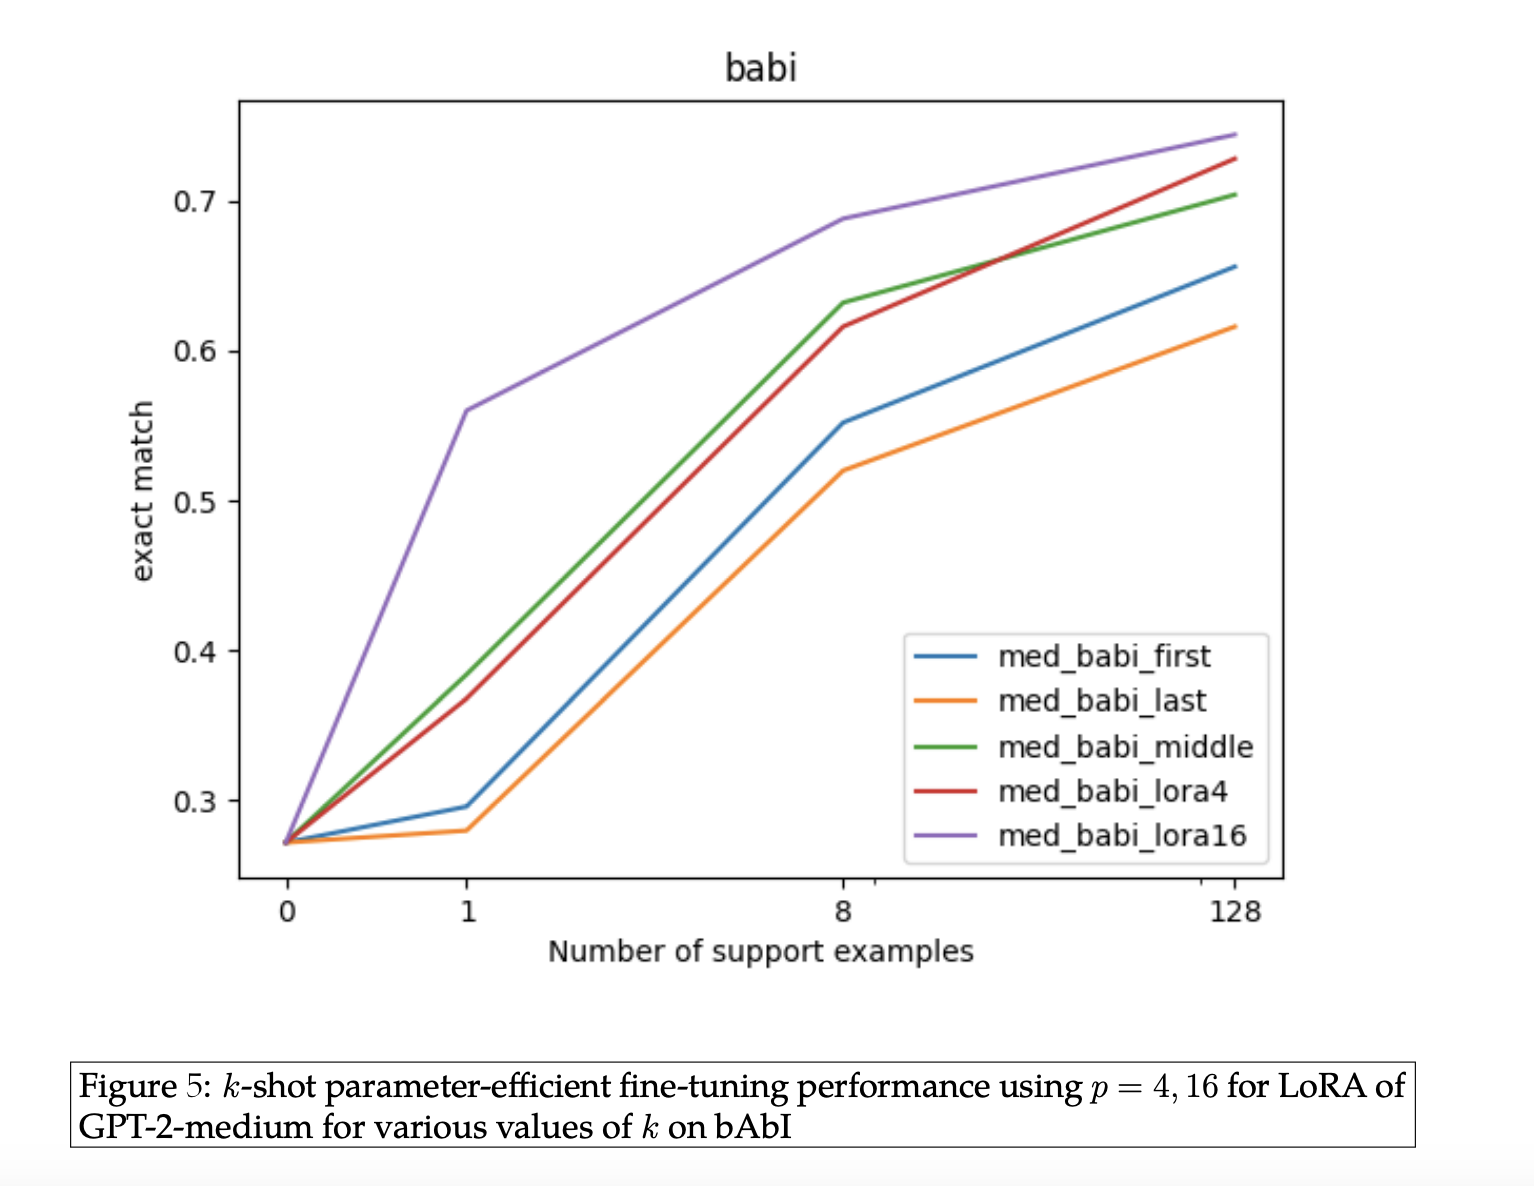
\includegraphics[width=0.75\linewidth]{./figures/parameter-3cii}
\end{center}

    \item \points{3dii} {\bf Reason on Fine-Tuning with LoRA}

Describe the results here.
\end{enumerate}
\end{enumerate}